\documentclass[a4paper,12pt]{article}
\usepackage[utf8]{inputenc}
\usepackage{graphicx}
\usepackage{fancyhdr}
\usepackage{lipsum}  % Nur zum Erzeugen von Beispieltext
\usepackage{hyperref}
\begin{document}

% Titelseite
\begin{titlepage}
    \centering
    % Bild einfügen
    
\includegraphics[width=0.8\textwidth]{uni-bielefeld-logo-1100x825.jpg}  % Ersetzen Sie 'bild.png' durch den Namen Ihres Bildes
    \vfill
    
    % Text unter dem Bild
    {\Huge Abgabe im Fach Computergestützte Methoden der Wirtschaftswissenschaften \par}
    \vskip 1cm
    {\Large zum Thema: \par}
    \vskip 0.5cm
    {\LARGE Datenverarbeitung-/haltung: Analyse der Daten der Station Adelphi St \& Myrtle Ave \par}
    \vfill
    {\Large Thanh Huyen Doan (4167966) und Abinaya Jeyachandiran          (4180990) \par} % Fügen Sie hier Ihren Namen ein
    {\large Gruppe 20 \par} % Geben Sie Ihre Gruppennummer an
    {\large 02. Dezember 2024 \par} % Geben Sie das Abgabedatum an
\end{titlepage}




% Titelseite
\newpage


% Inhaltsverzeichnis
\tableofcontents
% Abbildungsverzeichnis
\listoffigures
\newpage

% Kapitel: Der zentrale Grenzwertsatz
\section{Der zentrale Grenzwertsatz}
Der zentrale Grenzwertsatz (ZGS) ist ein fundamentales Resultat der Wahrscheinlichkeitstheorie, das die Verteilung von Summen unabhängiger, identisch verteilter (i.i.d.) Zufallsvariablen (ZV) beschreibt. Er besagt, dass unter bestimmten Voraussetzungen die Summe einer großen Anzahl solcher ZV annähernd normalverteilt ist, unabhängig von der Verteilung der einzelnen ZV. Dies ist besonders nützlich, da die Normalverteilung gut untersucht und mathematisch handhabbar ist.

\\subsection{Aussage}
Sei \( X_1, X_2, \ldots, X_n \) eine Folge von i.i.d. ZV mit dem Erwartungswert \( \mu = E(X_i) \)
und der Varianz \( \sigma^2 = \text{Var}(X_i) \), wobei \( 0 < \sigma^2 < \infty \) gelte. Dann konvergiert
die standardisierte Summe \( Z_n \) dieser ZV für \( n \to \infty \) in Verteilung gegen eine Standardnormalverteilung:%
\footnote{Der zentrale Grenzwertsatz hat verschiedene Verallgemeinerungen. Eine davon ist der Lindeberg-Feller-Zentrale-Grenzwertsatz [1, Seite 328], der schwächere Bedingungen an die Unabhängigkeit und die identische Verteilung der ZV stellt.}


\[
Z_n = \frac{\sum_{i=1}^n X_i - n\mu}{\sigma \sqrt{n}} \xrightarrow{d} N(0, 1).
\]
Das bedeutet, dass für große \( n \) die Summe der ZV näherungsweise normalverteilt ist mit Erwartungswert \( n\mu \) und Varianz \( n\sigma^2 \):

\[
\sum_{i=1}^n X_i \sim N(n\mu, n\sigma^2).
\]

\subsection{Erklärung der Standardisierung}
Um die Summe der ZV in eine Standardnormalverteilung zu transformieren, subtrahiert man den Erwartungswert \( n\mu \) und teilt durch die Standardabweichung \( \sigma \sqrt{n} \). Dies führt zu der obigen Formel. Die Darstellung (2) ist für \( n \to \infty \) nicht wohldefiniert.

\subsection{Anwendungen}
Der ZGS wird in vielen Bereichen der Statistik und der Wahrscheinlichkeitstheorie angewendet. Typische Beispiele sind:


\subsubsection{Anwendungsfall 1: Statistik}
Der zentrale Grenzwertsatz ist essenziell für die Anwendung von Hypothesentests und die Erstellung von Konfidenzintervallen.

\subsubsection{Anwendungsfall 2: Maschinelles Lernen}
Im Bereich des maschinellen Lernens wird der ZGS verwendet, um zufällige Schwankungen bei der Schätzung von Modellparametern zu analysieren.


\newpage

% Kapitel: Bearbeitung zur Aufgabe 1
\section{Bearbeitung zur Aufgabe 1}

\subsection{Datenverarbeitung}
\subsubsection{Untersuchung des gruppenspezifischen Datensatzes: Aufbau und Erkenntnisse}
Für die Analyse wurde der Datensatz der Station "Adelphi St \& Myrtle Ave", die unserer Gruppe 20 zugeordnet ist, untersucht. Der Datensatz enthält Informationen zum Fahrradverleih und zu den Wetterbedingungen im Zeitraum vom 1. Januar 2023 bis zum 31. Dezember 2023.
Jede Zeile des Datensatzes repräsentiert eine individuelle Aufzeichnung, wobei die relevanten Daten sich in den Zellen von A2 bis A36.440 befinden. Die Attributnamen, die in Zelle A1 aufgeführt sind, umfassen:
\begin{itemize}
    \item \texttt{date}: Das Datum der Aufzeichnung
    \item \texttt{station}: Der Name der Verleihstation
    \item \texttt{count}: Die Anzahl der ausgeliehenen Fahrräder
    \item \texttt{precipitation}: Niederschlagsmenge
    \item \texttt{windspeed}: Windgeschwindigkeit
    \item \texttt{min\_temperature}, \texttt{average\_temperature}, \texttt{max\_temperature}: Wetterinformationen zu minimalen, durchschnittlichen und maximalen Temperaturen
\end{itemize}
Unsere Analyse konzentriert sich insbesondere auf die Attribute \texttt{date}, \texttt{average\_temperature}, \texttt{max\_temperature}, \texttt{min\_temperature} und \texttt{count}, da diese essenziell sind, um den Einfluss der Wetterlage auf die Nutzungsmuster der Station zu untersuchen.

\paragraph{Erkenntnisse:}
\begin{itemize}
    \item Die Anzahl der Ausleihen variiert stark in Abhängigkeit von der Wetterlage. Besonders extreme Temperaturen oder Niederschlagsmengen korrelieren mit einer geringeren Anzahl an Ausleihen.
    \item Es wurden fehlende Werte in den Spalten \texttt{count} (Anzahl der Ausleihen) und \texttt{average\_temperature} (Durchschnittstemperatur) festgestellt. Diese müssen für eine präzise Analyse berücksichtigt oder entsprechend bereinigt werden.
\end{itemize}
Zusammenfassend zeigt der Datensatz eine klare Verbindung zwischen Wetterbedingungen und der Nutzung des Fahrradverleihsystems. Die Bereinigung und gezielte Analyse der relevanten Attribute wird in den nächsten Schritten fortgeführt.

\subsubsection{Import des Datensatzes in eine Tabellenkalkulation}
Der Datensatz wurde erfolgreich in eine Tabellenkalkulation (Microsoft Excel) importiert. Die Daten wurden in tabellarischer Form dargestellt, wobei die Spaltenüberschriften aus dem Datensatz übernommen wurden. Zur besseren Übersicht und Handhabung wurden Filter für alle Spalten aktiviert. Diese ermöglichen eine gezielte Sortierung und Filterung der Daten nach spezifischen Kriterien, wie z. B. Datum, Temperaturen oder Anzahl der Ausleihen.

Die Tabelle bietet damit eine klare Grundlage für die weiteren Analysen und Auswertungen. Abbildung~\ref{fig:data_table} zeigt den importierten Datensatz.

\begin{figure}[h!]
\centering
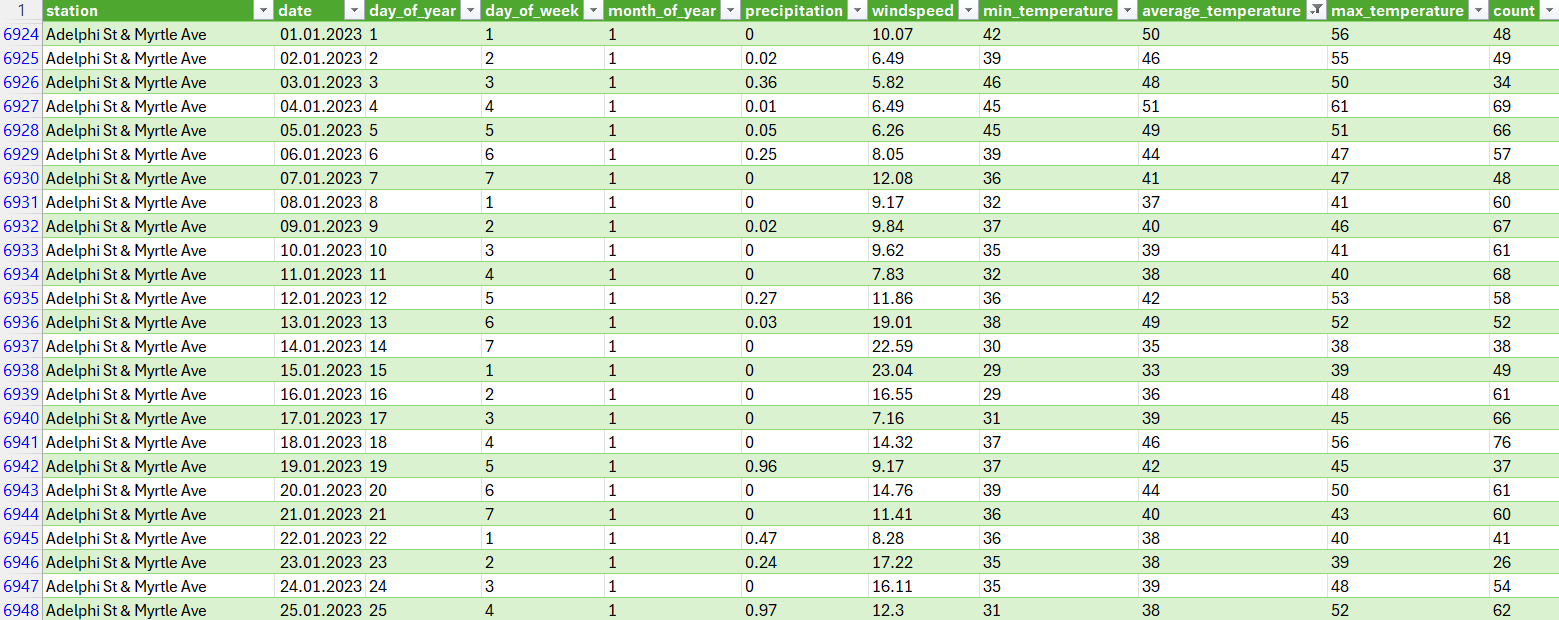
\includegraphics[width=0.8\textwidth]{20241201_18124556.png}
\caption{Importierte Wetter- und Verleihdaten mit Filteroptionen.}
\label{fig:data_table}
\end{figure}


\subsection{Berechnung der höchsten mittleren Temperatur in Grad Celsius}
Zur Berechnung der höchsten mittleren Temperatur wurde zunächst der Filter aktiviert und alle ungültigen Werte, wie beispielsweise „NA“, aus den Daten entfernt. Anschließend wurde mit der Funktion \texttt{MAX} der höchste mittlere Temperaturwert ermittelt, der 51 betrug. Dieser Wert wurde daraufhin von Fahrenheit in Celsius umgerechnet.


\begin{figure}[h!]
\centering
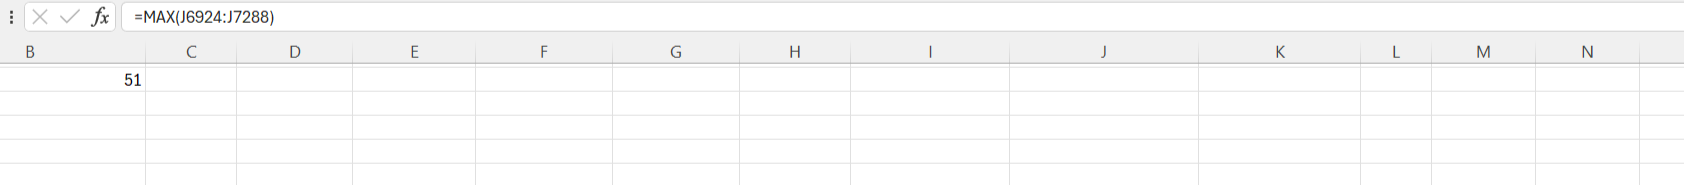
\includegraphics[width=0.8\textwidth]{20241201_18191811.png} % Bild einfügen
\caption{Excel-Befehl zur Berechnung des höchsten Wertes.}
\label{fig:excel_command}
\end{figure}
Nachdem der höchste mittlere Temperaturwert mit der \texttt{MAX}-Funktion ermittelt wurde, wurde dieser Wert von Fahrenheit in Celsius umgerechnet. Die Formel zur Umrechnung lautet:
\[
C = (F - 32) \cdot \frac{5}{9}
\]

Dabei ist \(F\) der ermittelte Wert in Fahrenheit und \(C\) der umgerechnete Wert in Celsius.

Im Folgenden ist der Prozess der Umrechnung von Fahrenheit in Grad Celsius abgebildet.

\begin{figure}[h!]
\centering
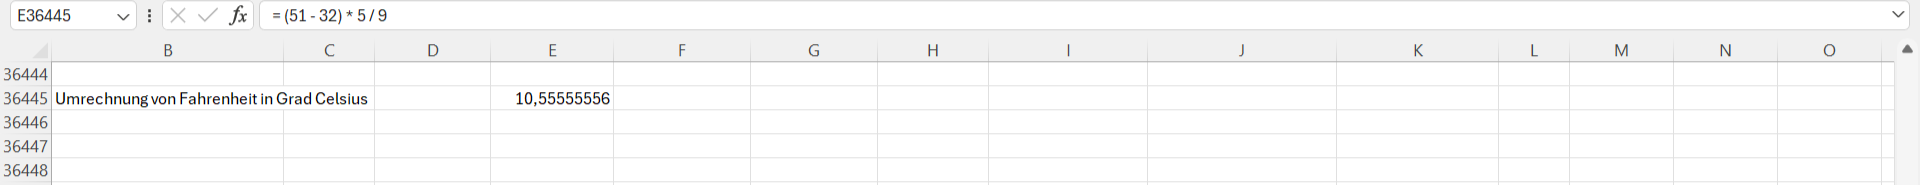
\includegraphics[width=0.8\textwidth]{20241201_18485367.png} % Bild einfügen
\caption{Umrechnung von Fahrenheit in Grad Celsius.}
\label{fig:fahrenheit_to_celsius}
\end{figure}


\subsection{Datenhaltung}
\subsubsection{Entwurf des Datenbank-Schemas unter Berücksichtigung der 1. und 2. Normalform}
\paragraph{Erste Normalform (1NF):}
Die Erste Normalform verlangt, dass alle Attribute atomar sind und jede Zeile durch einen eindeutigen Primärschlüssel identifiziert wird.


% Bild nach der ersten Normalform
\begin{figure}[h!]
\centering
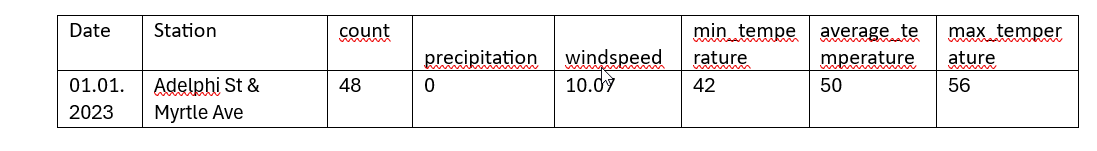
\includegraphics[width=0.8\textwidth]{20241202_01150744.png}  % Ersetzen Sie 'bild1.png' durch Ihren tatsächlichen Bildnamen
\caption{Beispiel zur ersten Normalform (1NF).}
\label{fig:bild1}
\end{figure}

\paragraph{Zweite Normalform (2NF):}
Die Zweite Normalform stellt sicher, dass alle Nicht-Schlüssel-Attribute vollständig vom gesamten Primärschlüssel abhängen und keine partiellen Abhängigkeiten existieren.

% Abbildung nach der zweiten Normalform
\begin{figure}[h!]
\centering
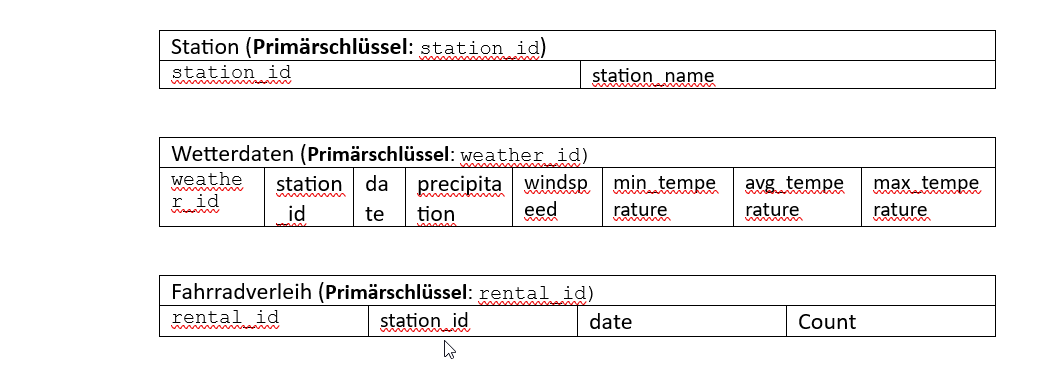
\includegraphics[width=0.8\textwidth]{20241202_01151045.png}  % Ersetzen Sie 'bild2.png' durch Ihren tatsächlichen Bildnamen
\caption{Beispiel zur zweiten Normalform (2NF).}
\label{fig:bild2}
\end{figure}

% Optionaler Seitenumbruch, damit der Text nicht über das Bild rutscht
\newpage



\subsubsection{Implementierung des Datenbankschemas in SQL}
% Drei Bilder untereinander
\begin{figure}[h!]
\centering
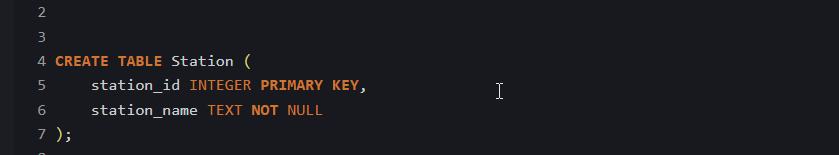
\includegraphics[width=0.8\textwidth]{20241201_19513817.png}  % Ersetzen Sie 'bild1.png' durch Ihren Bildnamen
\label{fig:bild1}
\end{figure}

\begin{figure}[h!]
\centering
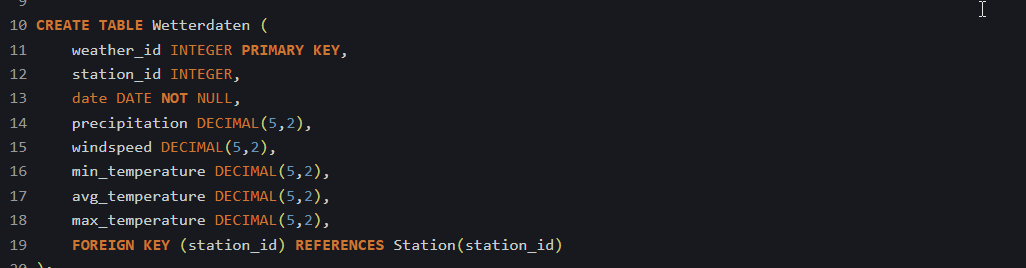
\includegraphics[width=0.8\textwidth]{20241201_19514551.png}  % Ersetzen Sie 'bild2.png' durch Ihren Bildnamen
\label{fig:bild2}
\end{figure}

\begin{figure}[h!]
\centering
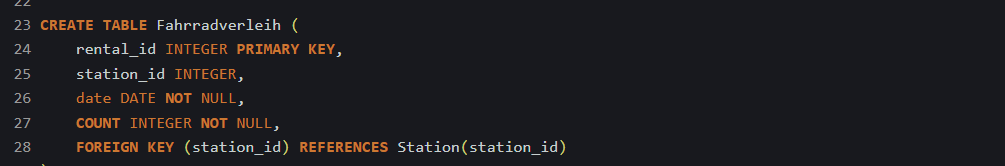
\includegraphics[width=0.8\textwidth]{20241201_19515000.png}  % Ersetzen Sie 'bild3.png' durch Ihren Bildnamen
\label{fig:bild3}
\end{figure}

% Text nach den Bildern
Die Umsetzung des Schemas in SQL (DDL) erfolgte durch die Erstellung von drei Tabellen, die den Datensatz sinnvoll strukturierten: eine Tabelle für die Stationen, eine für die Wetterdaten und eine für die Fahrradverleihvorgänge. Jede Tabelle wurde mit den notwendigen Attributen und Datenbeziehungen (wie Primär- und Fremdschlüsseln) definiert, um die Integrität und Konsistenz der Daten zu gewährleisten. Dabei wurde besonders auf die Normalisierung geachtet, um Redundanzen zu vermeiden und die Effizienz der Abfragen zu optimieren.Die SQL-Statements wurden präzise formuliert, um die Tabellen korrekt zu erstellen und eine einfache Datenpflege zu ermöglichen.
Der Datensatz wurde in Excel importiert, bereinigt und in drei Kategorien unterteilt: Stationen, Wetterdaten und Fahrradverleih. Jede Kategorie wurde in eine separate Tabelle überführt und mit einer eindeutigen ID für die Stationen versehen. Anschließend wurden die Daten als CSV-Dateien exportiert, um den Import in die SQL-Datenbank zu ermöglichen.

\subsection{SQL-Abfrage zur Ermittlung der höchsten mittleren Temperatur in Grad Celsius für die zugeordnete Station}

% Bild einfügen
\begin{figure}[h!]
\centering
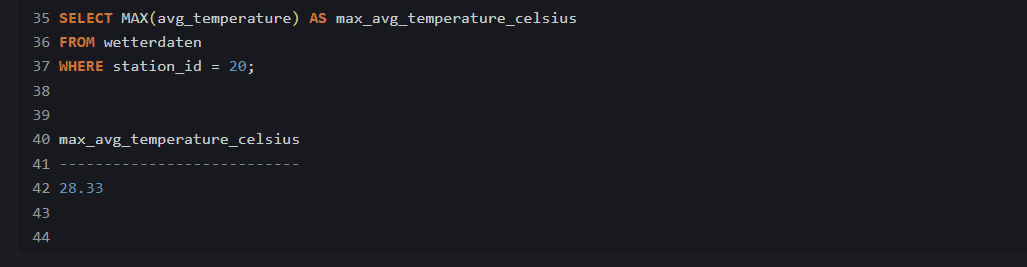
\includegraphics[width=0.8\textwidth]{20241201_20055471.png}  % Ersetzen Sie 'sql_query_image.png' durch Ihren Bildnamen
\caption{Abbildung der SQL-Abfrage zur Ermittlung der höchsten mittleren Temperatur.}
\label{fig:sql_query}
\end{figure}

% Text nach dem Bild
Die SQL-Abfrage dient dazu, die höchste mittlere Temperatur in Grad Celsius für die zugewiesene Station (Station 20) zu ermitteln. Dazu wird die \texttt{MAX()}-Funktion verwendet, um den höchsten Wert aus der Spalte \texttt{avg\_temperature} in der Tabelle \texttt{wetterdaten} zu extrahieren. Die \texttt{WHERE}-Klausel filtert die Datensätze und stellt sicher, dass nur die Werte für die Station mit der \texttt{station\_id = 20} berücksichtigt werden. Das Ergebnis dieser Abfrage liefert den höchsten durchschnittlichen Temperaturwert aus den relevanten Wetterdaten für diese Station.




\newpage

% Literaturverzeichnis
\begin{thebibliography}{9}
\bibitem{vorlage}
Achim Klenke. \textit{Wahrscheinlichkeitstheorie.} Springer, 3. Auflage, 2013.
\bibitem{overleaf} 
Overleaf. \textit{Overleaf - Online LaTeX Editor}, \url{https://www.overleaf.com/project/674cd2c7f7e5e5d86fcfa29a}.
\bibitem{sqlite} 
SQLite. \textit{SQLite Online}, \url{https://sqliteonline.com/}.
\end{thebibliography}

\section*{Abgabe des LaTeX-Codes}

Der für diese Abgabe zu erstellende LaTeX-Code wurde in einem GitHub-Repository zur Verfügung gestellt. Sie können den Commit des LaTeX-Codes über den folgenden Link aufrufen:

\href{https://github.com/winwin1309/Latex-COMET-Abgabe-1--Gruppe20/commit/c46b79784c59612828f0b85de1aa45dbfaeb9dc6}
{GitHub Commit Link}

Bitte klicken Sie auf den Link, um den spezifischen Commit des LaTeX-Codes zu sehen.

\end{document}
